\documentclass[12pt, letterpaper]{article}

\usepackage[english]{babel} % Sets the language and regional settings for English documents
\usepackage[utf8]{inputenc} % Allows the use of UTF-8 characters in the document
\usepackage[T1]{fontenc} % Specifies the font encoding
\usepackage[margin=2cm]{geometry} % Sets the page margins
\usepackage{makeidx} % Enables the creation of indexes
\usepackage{natbib} % Provides flexible bibliography support
\usepackage{url} % Allows the use of URLs
\usepackage{enumitem} % Customizes the appearance of lists
\usepackage{listings} % Provides syntax highlighting for code listings
\usepackage[dvipsnames]{xcolor} % Allows the use of colors
\usepackage{parskip} % Modifies paragraph spacing
\usepackage{graphicx} % Enables the inclusion of graphics
\usepackage{tikz} % Allows the creation of graphics and diagrams
\usepackage{float}
\usepackage{hyperref} % Enables the creation of hyperlinks
\usepackage{amsmath} % Provides additional math environments and commands
\usepackage{circuitikz} % Allows the creation of electrical circuits
\usepackage{adjustbox} % Adjusts the size of the circuit diagrams
\usepackage{arydshln} % Allows the use of dashed lines in tables
\usepackage{tcolorbox} % Allows the use of colored boxes

\definecolor{mygray}{gray}{0.9}
\usetikzlibrary{shapes.geometric, positioning}

\lstset{
	language=SQL,
	basicstyle=\ttfamily\small,
	keywordstyle=\color{blue},
	commentstyle=\color[rgb]{0,0.5,0},
	stringstyle=\color{red},
	numbers=left,
	numberstyle=\tiny\color{gray},
	stepnumber=1,
	numbersep=10pt,
	backgroundcolor=\color{white},
	showspaces=false,
	showstringspaces=false,
	breaklines=true,
	frame=single,
	tabsize=2, captionpos=b, lineskip=-1pt,
	extendedchars=true,
	literate={á}{{\'a}}1 {é}{{\'e}}1 {í}{{\'i}}1 {ó}{{\'o}}1 {ú}{{\'u}}1 {Á}{{\'A}}1 {É}{{\'E}}1 {Í}{{\'I}}1 {Ó}{{\'O}}1 {Ú}{{\'U}}1 {ñ}{{\~n}}1 {Ñ}{{\~N}}1 {¿}{{\textquestiondown}}1 {¡}{{\textexclamdown}}1
}

% VHDL language configuration
\lstdefinelanguage{VHDL}{
	morekeywords={entity, architecture, signal, port, in, out, inout, begin, end, process, if, then, else, elsif, case, when, others, for, while, loop, wait, library, use, std_logic, std_logic_vector, integer, boolean, rising_edge, falling_edge, component, generic, map, downto, to, and, or, not, xor, nand, nor, xnor},
	morecomment=[l]{--},
	morestring=[b]",
	sensitive=false,
	alsoletter={_}
}

% VHDL listings style
\lstdefinestyle{vhdl}{
	language=VHDL,
	basicstyle=\ttfamily\small,
	keywordstyle=\color{blue}\bfseries,
	commentstyle=\color[rgb]{0,0.6,0}\itshape,
	stringstyle=\color{red},
	numbers=left,
	numberstyle=\tiny\color{gray},
	stepnumber=1,
	numbersep=10pt,
	backgroundcolor=\color{white},
	showspaces=false,
	showstringspaces=false,
	breaklines=true,
	frame=single,
	tabsize=2,
	captionpos=b,
	lineskip=-1pt,
	extendedchars=true
}

\graphicspath{ {./img/} } % Sets the path for the graphics

\newlist{biblio}{enumerate}{1}
\setlist[biblio,1]{label=[\arabic*]}

\makeindex

\begin{document}

\begin{titlepage}

	\begin{tikzpicture}[remember picture,overlay]
		\node[anchor=north west, inner sep=30] at (current page.north west) {
			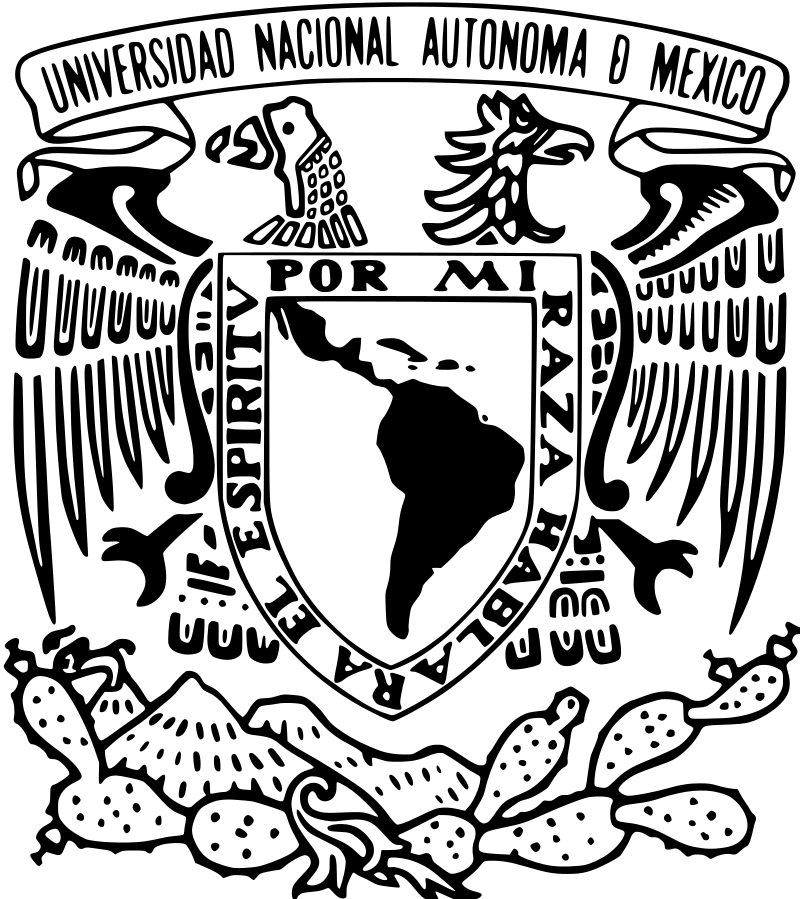
\includegraphics[width=4cm]{escudoUNAM.png}
		};

		\node[anchor=north east, inner sep=30] at (current page.north east) {
			
\includegraphics[width=4cm]{escudoFI.png}
		};
	\end{tikzpicture}

	\begin{center}
		\vspace*{3cm}

		\Huge
		\textbf{Práctica 2 - Análisis Senoidal de Circuitos Trifásicos Balanceados y Desbalanceados}

		\vspace{2.5cm}

		\Huge
		\textbf{Facultad de Ingeniería}\\
		Circuitos Eléctricos\\
		Semestre 2026-1\\

		\vspace{2.5cm}

		\textbf{Grupo:} 4

		\vspace{2.5cm}

		\Huge
		Ugartechea González Luis Antonio\\
		Tepal Brinseño Hansel Yael \\
		\textbf{Fecha de entrega:}
		\vspace{2.5cm}
	\end{center}

\end{titlepage}

\section{Objetivo}

\begin{itemize}
	\item Determinar experimentalmente las relaciones entre los voltajes de línea y voltajes de fase.
	\item Determinar experimentalmente las relaciones entre las corrientes de línea y las corrientes entre líneas.
	\item Verificar la relación entre el voltaje y la corriente en un inductor.
	\item Verificar la relación entre el voltaje y la corriente en un capacitor.
	\item Mediante el empleo de un simulador electrónico de un generador trifásico balanceado analizar prácticamente un circuito trifásico, empleando fasores.
\end{itemize}

\section{Introducción}

Un sistema trifásico balanceado es un método de generación y distribución de energía eléctrica formado por tres fuentes de tensión alterna de igual magnitud y frecuencia, desfasadas simétricamente 120° entre sí. Se considera balanceado cuando las impedancias de las cargas son idénticas en cada fase, resultando en corrientes de línea de igual magnitud. Los voltajes fundamentales son el voltaje de línea \(V_L\) (medido entre dos conductores de fase) y el voltaje de fase \(V_{\phi}\) (medido entre un conductor de fase y neutro), relacionados por \(V_L = \sqrt{3} \cdot V_{\phi}\) en conexión estrella (Y).

Las corrientes se clasifican en corriente de línea \(I_L\) (que fluye por los conductores de fase) y corriente de fase \(I_{\phi}\) (que circula por cada elemento de carga). En conexión estrella, \(I_L = I_{\phi}\), mientras que en conexión delta, \(I_L = \sqrt{3} \cdot I_{\phi}\). El ángulo de desfasamiento de 120° entre fases permite la creación de campos magnéticos giratorios en motores y asegura una entrega de potencia constante, siendo el estándar para transmisión de energía a gran escala debido a su eficiencia.

\section{Desarrollo}

\subsection{Experimento 1}

\begin{figure}[H]
	\centering
	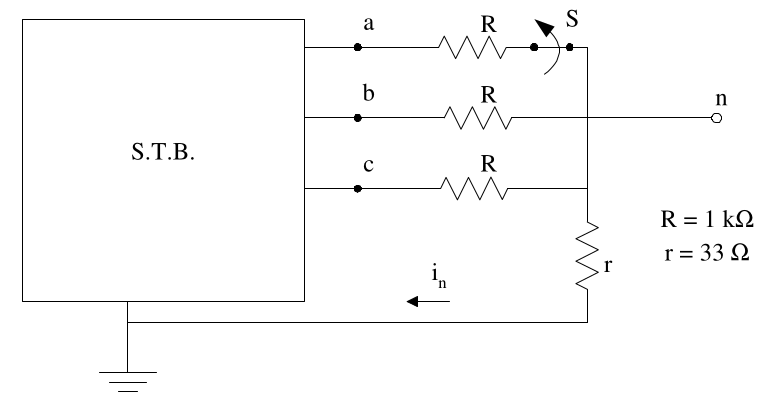
\includegraphics[width=0.6\textwidth]{circuito_exp1.png}
	\caption{Circuito del Experimento 1}
\end{figure}

a) Observe  con  el  interruptor  S  cerrado  las  formas  de  onda  correspondientes  a  los  voltajes  \(V_{ab}\) y \(V_{bn'}\), para efectuar las observaciones, conecte la tierra del osciloscopio en la terminal b y los canales A y B del osciloscopio en las terminales a y n' respectivamente (desconectando la tierra del osciloscopio de la tierra del ciruito). Dibuje los fasores correspondientes a \(V_{ab}\) y \(V_{bn'}\). Cual es la razón \(\frac{|V_{ab}|}{|V_{bn'}|}\)?

\textbf{Considere:} \(V_a = 0^\circ\)

\subsubsection*{Datos del STB práctico}

\begin{itemize}
	\item \(A = 6 V\) (Voltaje de fase)
	\item \(f = 685.129 Hz\) (Frecuencia)
\end{itemize}

\subsubsection*{Datos medidos del osciloscopio}

\begin{figure}[H]
	\centering
	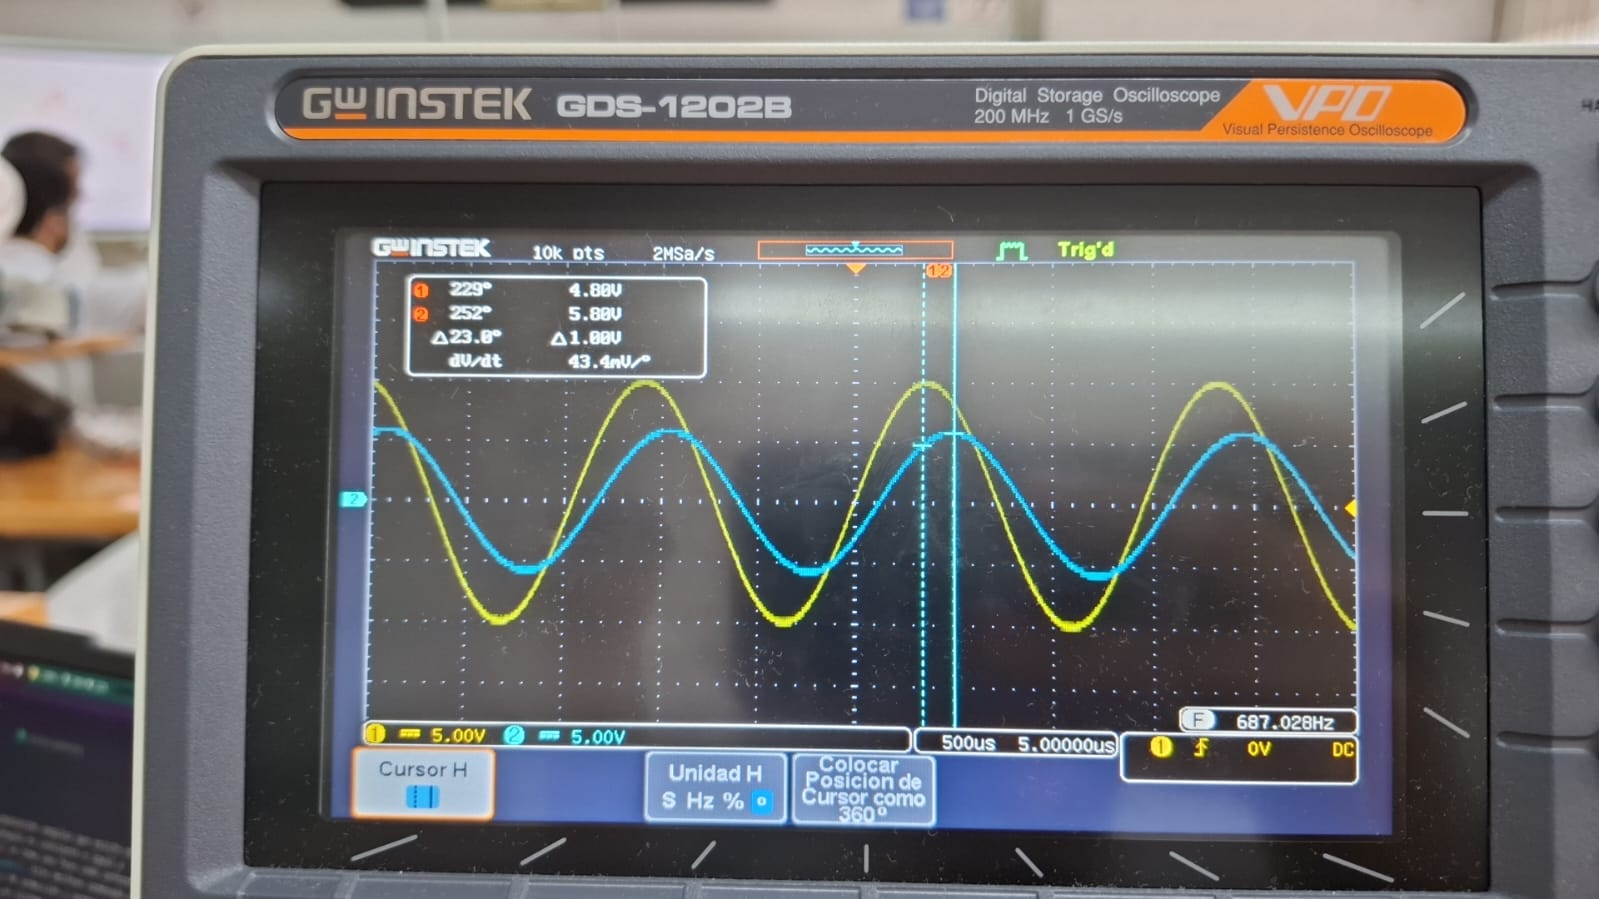
\includegraphics[width=0.6\textwidth]{Experimento1.jpeg}
	\caption{Datos medidos del osciloscopio}
\end{figure}
Del osciloscopio obtenemos el desfase entre A y B:

\begin{tcolorbox}[colback=mygray, colframe=LimeGreen, boxrule=0.7pt, arc=2pt, boxsep=1pt, left=2pt, right=2pt, top=2pt, bottom=2pt, title=Forma más reducida]

	\[ \phi_{AB} = \frac{t}{T} \cdot 360^{\circ} =\frac{(125x10^{-6})(360^{\circ})}{(1.45x10^{-3})} = 31.0344^\circ \]

\end{tcolorbox}

Y para la relación de voltajes a partir de los datos del osciloscopio donde tenemos:

\begin{itemize}
	\item \(V_{ab} = 10 [V_p]\)
	\item \(V_{bn'} = 5.25 [V_p]\)
\end{itemize}

\begin{tcolorbox}[colback=mygray, colframe=LimeGreen, boxrule=0.7pt, arc=2pt, boxsep=1pt, left=2pt, right=2pt, top=2pt, bottom=2pt, title=Forma más reducida]

	\[ V = \left| \frac{V_{ab}}{V_{bn'}} \right| = \left| \frac{10 V}{5.25 V} \right| = 1.90476 [V]\]

\end{tcolorbox}

\subsubsection{Error experimental}

Sabiedo que la relación teórica entre el voltaje de línea y el voltaje de fase es:
\[ V_L = \sqrt{3} \cdot V_{\phi} \]

Entonces podemos calcular el error experimental obtenido en la práctica:

\[ \text{Error} = \left| \frac{V_{L_{teorico}} - V_{L_{practico}}}{V_{L_{teorico}}} \right| \times 100\% \]

\[\text{Error} = \left| \frac{\sqrt{3} - 1.90476 V}{\sqrt{3}} \right| \times 100\% \]

\begin{tcolorbox}[colback=mygray, colframe=LimeGreen, boxrule=0.7pt, arc=2pt, boxsep=1pt, left=2pt, right=2pt, top=2pt, bottom=2pt, title=Forma más reducida]

	\[\text{Error} = 9.91\% \]

\end{tcolorbox}

De igual forma conocemos que el desfase teorico para este tipo de circuito es de \(30^\circ\), por lo que podemos calcular el error experimental del desfase:

\[ \text{Error} = \left| \frac{\phi_{teorico} - \phi_{practico}}{\phi_{teorico}} \right| \times 100\% \]

\[\text{Error} = \left| \frac{30^\circ - 31.0344^\circ}{30^\circ} \right| \times 100\% \]

\begin{tcolorbox}[colback=mygray, colframe=LimeGreen, boxrule=0.7pt, arc=2pt, boxsep=1pt, left=2pt, right=2pt, top=2pt, bottom=2pt, title=Forma más reducida]

	\[\text{Error} = 3.45\% \]

\end{tcolorbox}


\subsubsection{Fasores}

\begin{figure}[H]
	\centering
	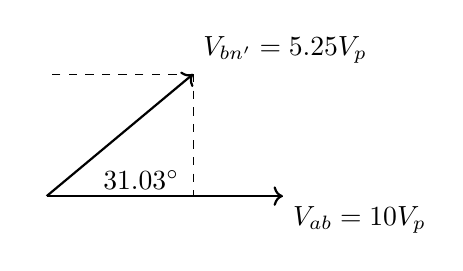
\begin{tikzpicture}
		\draw[->, thick] (0,0) -- (3,0) node[anchor=north west] {\(V_{ab} = 10 V_p\)};
		\draw[->, thick] (0,0) -- (1.86,1.55) node[anchor=south west] {\(V_{bn'} = 5.25 V_p\)};
		\draw[dashed] (1.86,1.55) -- (1.86,0) node[anchor=north west] {};
		\draw[dashed] (1.86,1.55) -- (0,1.55) node[anchor=north east] {};
		\draw[dashed] (3,0) -- (1.86,0);
		\draw[dashed] (3,0) -- (0,0);
		\node at (1.2, 0.2) {\(31.03^\circ\)};
	\end{tikzpicture}
	\caption{Fasores de \(V_{ab}\) y \(V_{bn'}\)}
\end{figure}

b) Observe con el interruptor cerrado el voltaje correspondiente a la resistencia \(r\).

c) Observe con el interruptor abierto el voltaje correspondiente a la resistencia \(r\).

d) ¿Qué concluye de los incisos b) y c) anteriores con respecto a la corriente \(i_n\)?

En base a los datos obtenidos en el osciloscopio, podemos observar que el voltaje a través de la resistencia \(r\) permanece prácticamente constante tanto con el interruptor cerrado como abierto. Esto indica que la corriente \(i_n\) a través de la resistencia \(r\) no se ve afectada significativamente por el estado del interruptor.

Esto se debe en parte a que en un sistema trifásico balanceado, la corriente de línea y la corriente de fase están relacionadas de manera que la desconexión de una carga (en este caso, el interruptor) no altera sustancialmente las condiciones de operación de las otras fases. La resistencia \(r\) sigue recibiendo la misma cantidad de corriente debido a la simetría del sistema y la distribución equilibrada de las cargas.

\subsection{Experimento 2}

\begin{figure}[H]
	\centering
	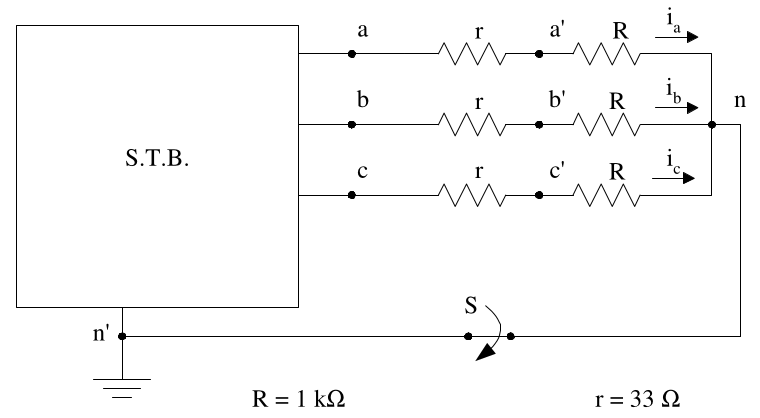
\includegraphics[width=0.6\textwidth]{circuito_exp2.png}
	\caption{Circuito del Experimento 2}
\end{figure}

a) Conecte  la  tierra  del  osciloscopio  a  la  terminal a' y los canales A y B a  las  terminales  a  y  n respectivamente. En el canal A se observará la forma de onda asociada a la corriente \(i_a\)  y en el canal B se observará  la  forma  de  onda  correspondiente  al voltaje \(V_{a'n}\) desfasada 180°. Determine los fasores correspondientes a \(I_a\) y \(V_{a'n}\).

\subsection*{Datos del STB práctico}

\begin{itemize}
	\item \(A = 6 V\) (Voltaje de fase)
	\item \(f = 685.129 Hz\) (Frecuencia)
\end{itemize}

\subsubsection{Mediciones del osciloscopio}
\begin{figure}[H]
	\centering
	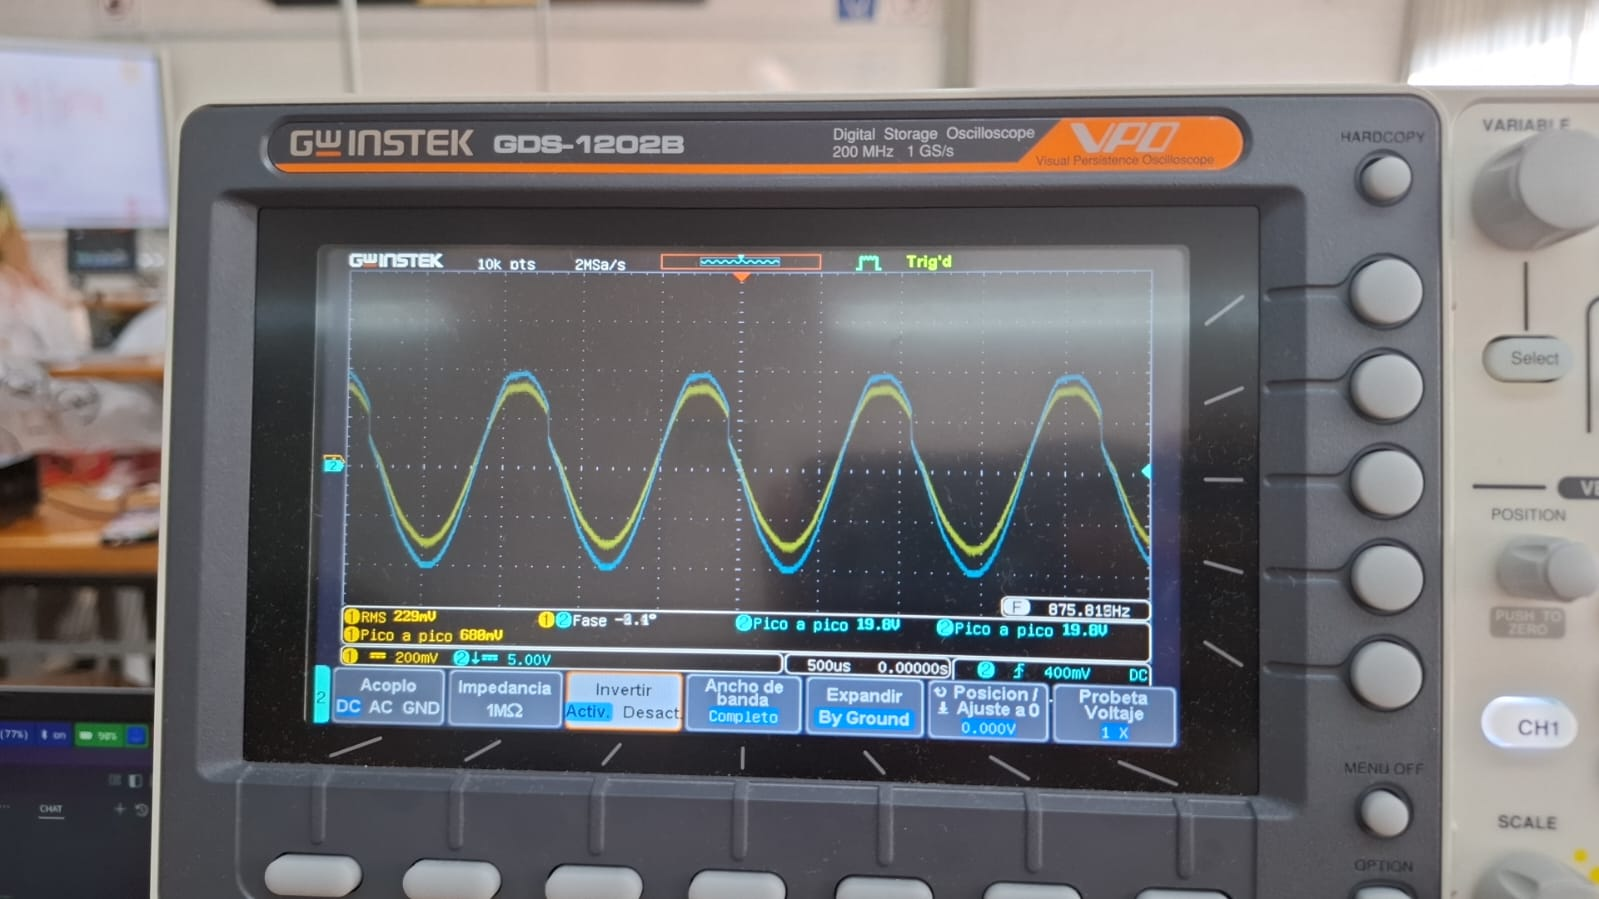
\includegraphics[width=0.6\textwidth]{Exp2_canalBinvertido.jpeg}
	\caption{Mediciones del osciloscopio}
\end{figure}

\subsection*{Para la corriente de línea con el switch cerrado de \(r_A\)}

\textbf{Donde:}

\begin{itemize}
	\item \(V_{L_{r_A}} = 312 [mV_p]\)
	\item \(V_{\phi_{r_A}} = 9.4 [V_p]\)
	\item \(R_{r_A} = 33 [\Omega]\)
	\item \(\Phi = 2.4^\circ\)
\end{itemize}

Utilizando la ley de Ohm:

\begin{itemize}
	\item \(I_{r_A} = \frac{V_{L_{r_A}}}{R_{r_A}} = \frac{312 \times 10^{-3}}{33} = 9.4545 [mA]\)
\end{itemize}

Determinando la relación de la corriente y el voltaje:

\[\frac{I_a}{V_a'n} = \frac{9.4545 \times 10^{-3}}{6} \approx 1.5758 \times 10^{-3}\]

Fasor calculado:

\begin{tcolorbox}[colback=mygray, colframe=LimeGreen, boxrule=0.7pt, arc=2pt, boxsep=1pt, left=2pt, right=2pt, top=2pt, bottom=2pt, title=Forma más reducida]

	\[\frac{I_a}{V_a'n} = 1.5758 m[A/V]\]
	\[\phi = 2.4^\circ\]
\end{tcolorbox}

%Para dibujar los fasores como no hay desfase uno queda encima de otro

b) Efectúe las mediciones del inciso anterior con el interruptor S abierto.

\begin{figure}[H]
	\centering
	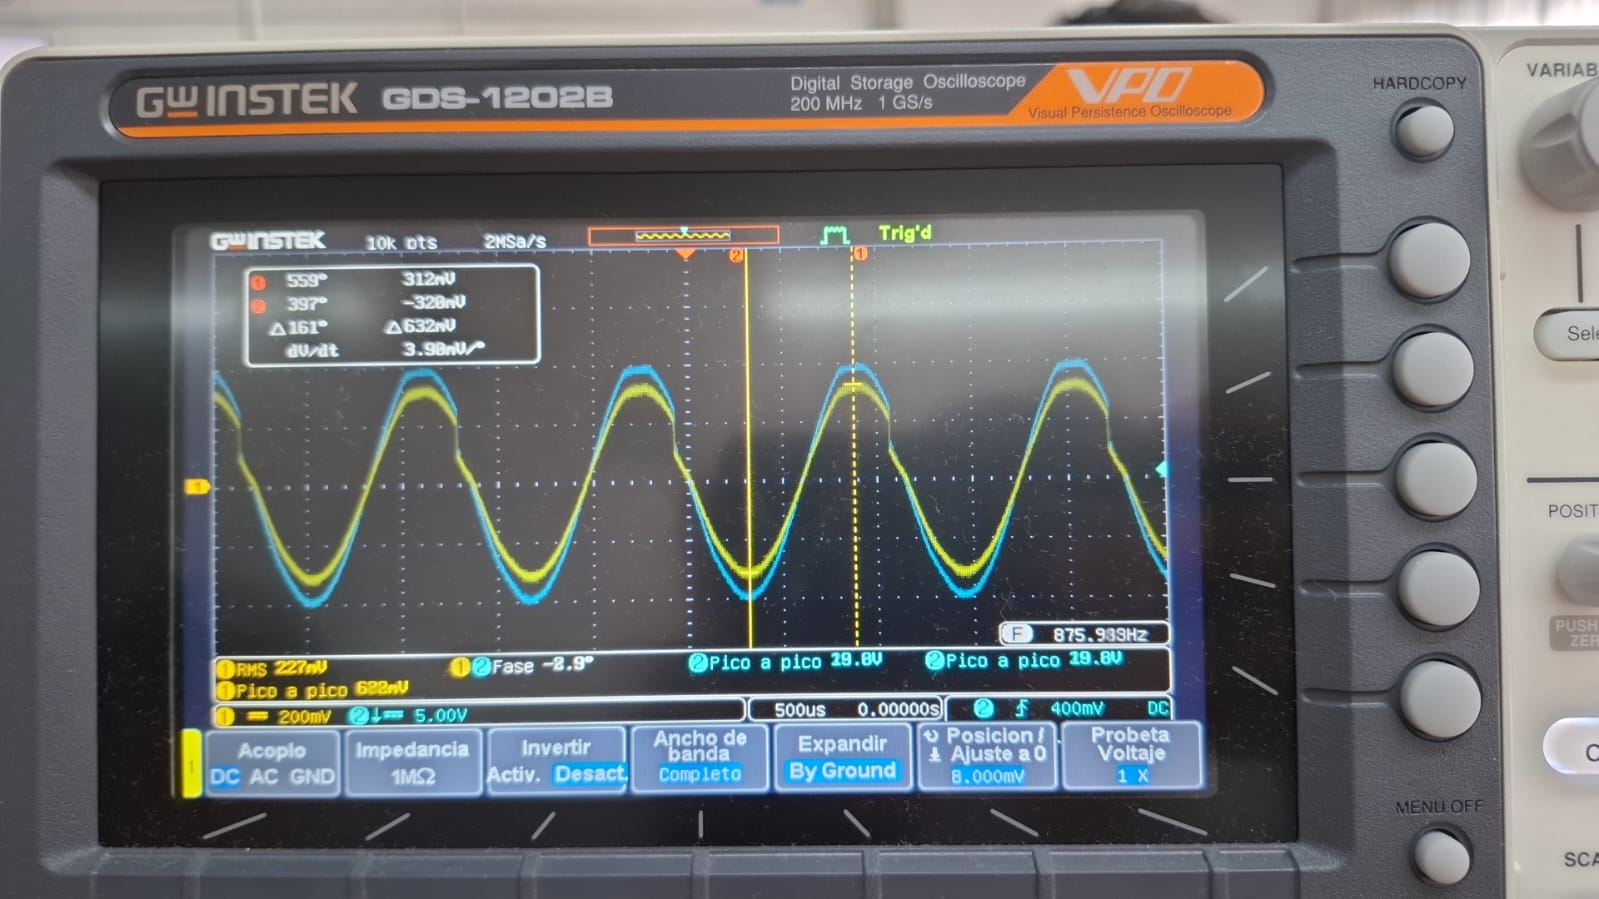
\includegraphics[width=0.6\textwidth]{Exp2_SwitchAbierto.jpeg}
	\caption{Mediciones del osciloscopio con switch abierto}
\end{figure}

% \begin{tikzpicture}
% 	\draw[->, thick] (0,0) -- (3,0) node[anchor=north west] {9.4 V};
% 	\draw[->, thick] (0,0) -- (0,3) node[anchor=south west] {9.4545 mA};
% \end{tikzpicture}

\subsection*{Para la corriente de línea con el switch abierto de \(r_A\)}

No varía mucho porque estamos manejando \(mV\) y al ser un sistema trifásico balanceado las corrientes son similares.

\begin{itemize}
	\item \(V_{L_{r_A}} = 312 [mV_p]\)
	\item \(V_{\phi_{r_A}} = 9.4 [V_p]\)
	\item \(R_{r_A} = 33 [\Omega]\)
	\item \(\Phi = 2.9^\circ\)
\end{itemize}

Utilizando la ley de Ohm:

\begin{itemize}
	\item \(I_{r_A} = \frac{V_{L_{r_A}}}{R_{r_A}} = \frac{312 \times 10^{-3}}{33} = 9.4545 [mA]\)
\end{itemize}

Fasor calculado:

\begin{tcolorbox}[colback=mygray, colframe=LimeGreen, boxrule=0.7pt, arc=2pt, boxsep=1pt, left=2pt, right=2pt, top=2pt, bottom=2pt, title=Forma más reducida]

	\[\frac{I_a}{V_a'n} = 1.5758 m[A/V]\]
	\[\phi = 2.4^\circ\]
\end{tcolorbox}

% \begin{tikzpicture}
% 	\draw[->, thick] (0,0) -- (3,0) node[anchor=north west] {9.4 V};
% 	\draw[->, thick] (0,0) -- (0,3) node[anchor=south west] {9.4545 mA};
% \end{tikzpicture}

c) ¿Qué concluye acerca de lo observado en los dos incisos anteriores?

\subsection*{Análisis de resultados}

Como se puede observar en las mediciones realizadas, los valores de voltaje y corriente se mantienen prácticamente constantes tanto con el switch cerrado como abierto. Esta estabilidad en las mediciones confirma las características fundamentales de un sistema trifásico balanceado:

\begin{itemize}
	\item La corriente de línea permanece en 9.4545 mA independientemente del estado del switch
	\item El voltaje de fase se mantiene estable en 9.4 V
	\item La variación mínima observada es atribuible a la precisión de los instrumentos de medición
\end{itemize}

Este comportamiento valida la teoría de que en un sistema trifásico balanceado, la desconexión de una carga no afecta significativamente las condiciones de operación de las otras fases, debido a la simetría del sistema y la distribución equilibrada de las cargas.

\subsubsection{Comparación entre los fasores del switch cerrado y abierto}

Al existir un desfase de \(2.4^\circ\) con el switch cerrado y \(2.9^\circ\) con el switch abierto, podemos observar que la diferencia es mínima, lo que indica que la apertura del switch no afecta significativamente el ángulo de fase entre la corriente y el voltaje en este sistema trifásico balanceado.

\begin{figure}[H]
	\centering
	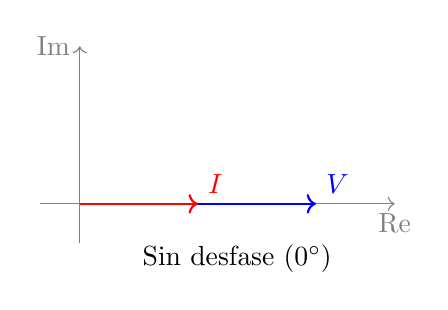
\begin{tikzpicture}
		% Ejes del plano cartesiano
		\draw[->, thin, gray] (-0.5,0) -- (4,0) node[anchor=north] {Re};
		\draw[->, thin, gray] (0,-0.5) -- (0,2) node[anchor=east] {Im};
		% Fasores alineados (sin desfase)
		\draw[->, thick, blue] (0,0) -- (3,0) node[anchor=south west] {\(V\)};
		\draw[->, thick, red] (0,0) -- (1.5,0) node[anchor=south west] {\(I\)};
		% Indicación de que no hay desfase
		\node at (2, -0.7) {Sin desfase (\(0^\circ\))};
	\end{tikzpicture}
	\caption{Fasores con switch cerrado - Sin desfase}
\end{figure}

\subsection{Experimento 3}

\begin{figure}[H]
	\centering
	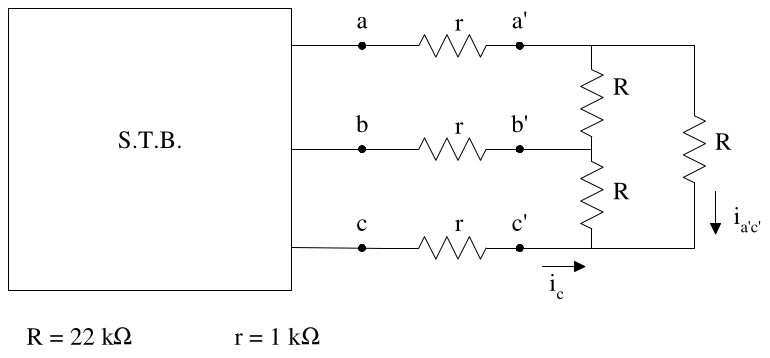
\includegraphics[width=0.6\textwidth]{circuito_exp3.png}
	\caption{Circuito del Experimento 3}
\end{figure}

a) Conecte la tierra del osciloscopio a la terminal c’ y los canales A y B a las terminales c y a’. Las formas de onda observadas serán proporcionales a las corrientes \(i_c\) y \(i_{a'c'}\) respectivamente.

\begin{figure}[H]
	\centering
	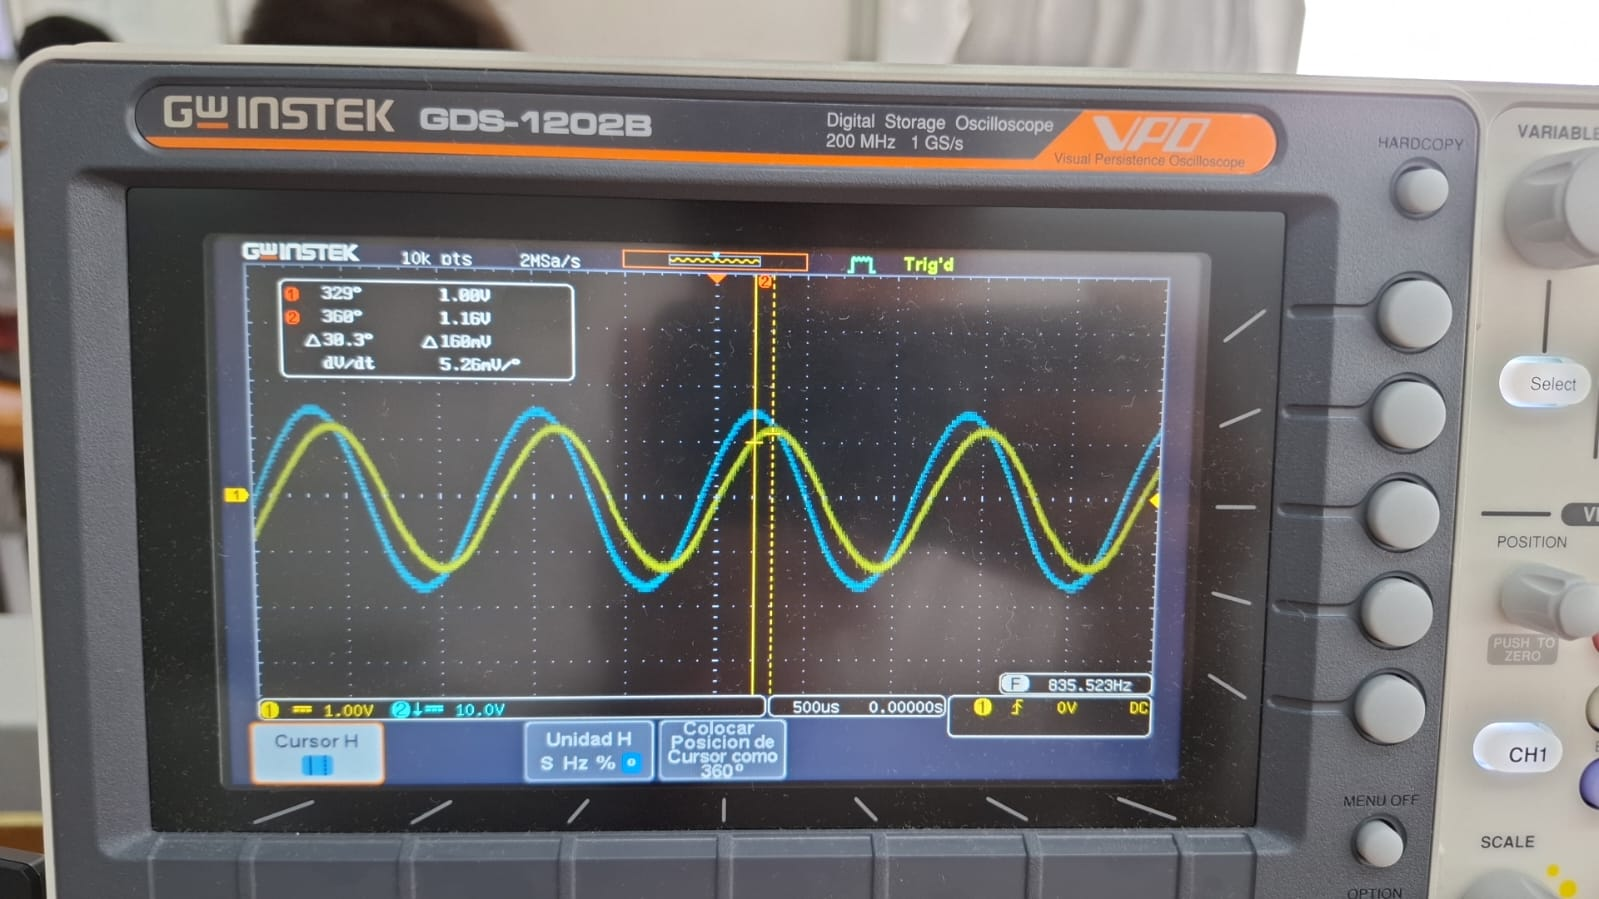
\includegraphics[width=0.6\textwidth]{Exp3_GradoDesfase.jpeg}
	\caption{Mediciones del osciloscopio}
\end{figure}

b) Conocidos los valores de las resistencias en el circuito, calcule la razón \(\frac{|I_{c'a'}|}{|I_c|}\).
\subsubsection*{Ángulo de desfase práctico}

\[\phi = 30.3^\circ \]

\subsubsection*{Voltaje de línea práctico}

\[ V_{L_{r_C}} = 1.36 V \]

\[ V_{L_{a'-c'}} = 15.6 V \]

\subsubsection*{Corriente de línea práctico}

\[ I_{c'} = 1.38 mA \]
\[ I_{a'-c'} = 0.7 mA \]

\subsubsection*{Para la corriente \(I_{c}\) y \(I_{a'-c'}\)}

\textbf{Donde:}

\begin{itemize}
	\item \(V_{L_{r_C}} = 1.36 [V_p]\)
	\item \(V_{L_{a'-c'}} = 15.6 [V_p]\)
	\item \(R = 22 [k\Omega]\)
	\item \(r = 1 [k\Omega]\)
\end{itemize}

\subsection{Cálculos de corriente}

Para \(I_{c'}\) tenemos:

\[I_{c'} = \frac{1.36 V}{1 k \Omega} = 1.36 mA\]

Para \(I_{a'-c'}\) tenemos:

\[I_{a'-c'} = \frac{15.6 V}{22 k \Omega} = 0.71 mA\]

Y la relación \textbf{\(\frac{|I_{c'-a'}|}{|I_c|}\)} es:

\[\frac{|I_{c'-a'}|}{|I_c|} = \frac{0.71 mA}{1.36 mA} = 0.522\]

\subsubsection*{Error experimental}

\[\text{Error} = \left| \frac{1.36 mA - 1.38 mA}{1.36 mA} \right| \times 100\% = 1.47\% \]

\begin{tcolorbox}[colback=mygray, colframe=LimeGreen, boxrule=0.7pt, arc=2pt, boxsep=1pt, left=2pt, right=2pt, top=2pt, bottom=2pt, title=Forma más reducida]
\[\text{Error} = 1.47\% \]
\end{tcolorbox}

\[\text{Error} = \left| \frac{0.71 mA - 0.7 mA}{0.71 mA} \right| \times 100\% = 1.41\% \]

\begin{tcolorbox}[colback=mygray, colframe=LimeGreen, boxrule=0.7pt, arc=2pt, boxsep=1pt, left=2pt, right=2pt, top=2pt, bottom=2pt, title=Forma más reducida]
\[\text{Error} = 1.41\% \]
\end{tcolorbox}

c) Considerando \(I_c = 0^\circ\), dibuje los fasores correspondientes a \(I_c\) e \(I_{a'c'}\).

\begin{figure}[H]
	\centering
	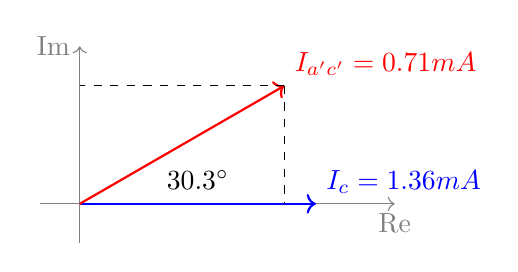
\begin{tikzpicture}
		% Ejes del plano cartesiano
		\draw[->, thin, gray] (-0.5,0) -- (4,0) node[anchor=north] {Re};
		\draw[->, thin, gray] (0,-0.5) -- (0,2) node[anchor=east] {Im};
		% Fasores con desfase
		\draw[->, thick, blue] (0,0) -- (3,0) node[anchor=south west] {\(I_c = 1.36 mA\)};
		\draw[->, thick, red] (0,0) -- (2.6,1.5) node[anchor=south west] {\(I_{a'c'} = 0.71 mA\)};
		% Indicación del ángulo de desfase
		\draw[dashed] (2.6,1.5) -- (2.6,0);
		\draw[dashed] (2.6,1.5) -- (0,1.5);
		\node at (1.5, 0.3) {\(30.3^\circ\)};
	\end{tikzpicture}
	\caption{Fasores de \(I_c\) e \(I_{a'-c'}\)}
\end{figure}

\section{Conclusiones}

\subsection{Hansel Yael Tepal Briseño}

A lo largo de la práctica se comprobó experimentalmente la relación teórica entre los voltajes y corrientes de línea y de fase en sistemas trifásicos balanceados. Las mediciones mostraron que el voltaje de línea es aproximadamente $\sqrt{3}$ veces el voltaje de fase y que la corriente de línea se mantiene prácticamente constante, validando la simetría y estabilidad de estos sistemas. Los errores experimentales fueron bajos, lo que respalda la precisión de los resultados y la correcta aplicación de la teoría.

Estos resultados también permitieron observar que la desconexión de una carga no afecta significativamente las condiciones de operación de las otras fases, confirmando la robustez de los sistemas trifásicos balanceados. El uso de fasores y el análisis de desfases entre voltaje y corriente facilitaron la comprensión del comportamiento de los circuitos, cumpliendo así con los objetivos planteados y reforzando la importancia de este tipo de análisis en la ingeniería eléctrica.

\subsection{Luis Antonio Ugartechea González}

La práctica permitió profundizar en la relación existente entre las magnitudes eléctricas de un sistema trifásico, mostrando que las condiciones teóricas de voltajes y corrientes se ven reflejadas con gran precisión en los resultados experimentales. La estabilidad observada en las mediciones respalda la eficiencia de los sistemas balanceados y su importancia en la transmisión y distribución de energía.

Además, se evidenció que la estructura simétrica de estos circuitos proporciona un funcionamiento confiable incluso ante la desconexión parcial de cargas. El empleo de representaciones fasoriales y el análisis del desfase entre señales resultaron fundamentales para interpretar adecuadamente el comportamiento del sistema, cumpliendo los objetivos planteados y destacando la relevancia de estas herramientas en la práctica de la ingeniería eléctrica.

% \section{Bibliography}

% \begin{biblio}
% 	%for: https://www.poli.edu.co/blog/poliverso/diseno-digital-que-es
% 	\item \textit{Diseño digital: qué es y por qué es importante.} (2021, August 26). Poliverso. Retrieved October 16, 2024, from: \textcolor{blue}{\underline{\url{https://www.poli.edu.co/blog/poliverso/diseno-digital-que-es}}}
% 	%for: https://www.sky6cancun.com/marketing/diseno-grafico/diseno-digital-que-es-y-para-que-sirve/
% 	\item \textit{Diseño digital: qué es y para qué sirve.} (2021, August 26). Sky6Cancún. Retrieved October 16, 2024, from: \textcolor{blue}{\underline{\url{https://www.sky6cancun.com/marketing/diseno-grafico/}}}
% \end{biblio}

\end{document}
